\section{Metodología}\label{metodologia}

Dado que PCMI pertenece a la categoría de problemas $\mathcal{NP}$-hard, en este trabajo se busca dar soluciones de la mejor calidad posible, pero no las óptimas. A continuación se presentan los distintos métodos utilizados para desarrollar algoritmos que lo resuelvan.

\section{Heurísticas constructivas golosas}

Las \textbf{heurísticas constructivas} son métodos que construyen iterativamente una solución factible para una instancia de un problema dado. Se suelen utilizar procedimientos golosos, que si bien no garantizan que las soluciones sean óptimas, retornan soluciones de una calidad aceptable por un costo computacional comparativamente menor. En este trabajo se implementa una heurística existente para el problema de coloreo \textit{(Secuencial - Largest First)} y se definen dos nuevas específicas para PCMI (\textit{Wyrnística Diferencial y Wyrna Power}).

\subsection{Secuencial - Largest First (S-LF)}

La heurística \textbf{secuencial} consiste en recorrer los vértices de forma secuencial y colorear a cada uno con el mínimo posible. La implementación \textbf{Secuencial - Largest First (LF)} los recorre en forma descendiente según su grado, lo cuál hace que genere coloreos más cercanos al óptimo. Es la heurística más natural para colorear los vértices de un grafo y su correctitud es trivial. Es fácil verificar que no genera siempre el coloreo óptimo, lo cual no resulta importante para PCMI dado que sólo interesa optimizar el impacto. En la \cref{fig:slf_coloreo} se presenta el coloreo obtenido con esta heurística.

El Algoritmo~\ref{alg:alg_secuencial} muestra una implementación posible. Es importante notar que es un algoritmo que solo toma en cuenta el grafo $G$ y no considera el impacto que genera. Sin embargo, resulta intuitivo que a menor cantidad de colores, mayor es la probabilidad de que haya un impacto alto.

\begin{algorithm}[H]
    \begin{algorithmic}[1]
        \State{\textbf{Entrada:} los grafos $G$ y $H$ en representación de listas de adyacencias}
        \State{\textbf{Salida:} coloreo de $G$ e impacto}
        \State
        \Function{$secuencialLF$}{$G$, $H$}:
            \State{$vertices \leftarrow \forall v \in G$ pares de $(d_G(v), v)$} \Comment{$O(n)$}
            \State{$sort(vertices)$}\Comment{$O(n\times log(n))$}
            
            \State{$coloreo \leftarrow array_n[undefined$]} \Comment{$O(n)$}
            
            \For{$(g,v)$ \textbf{in} $vertices$}: \Comment{$O(n^2)$}
                \For{$color~c$ \textbf{in} $1..n \wedge coloreo[v]~is~undefined$}:
                     \If{$\nexists\ u \in N_G(v) \mid coloreo[u] = c$} \Comment{$O(n)$}
                            \State{$coloreo[v] = c$}
                        \EndIf
                \EndFor
            \EndFor
    
            \State{\textbf{return} $coloreo$, $impacto(H,coloreo)$} \Comment{$O(m_H)$}
        \EndFunction
        \State{}
        \State{\textbf{Complejidad:} $O(n^2 + n\times log(n)+n + m_H) = O(n^2)$}
    \end{algorithmic}
    \caption{Algoritmo de \textit{Secuencial con ordenamiento Largest First} para PCMI.}
    \label{alg:alg_secuencial}
\end{algorithm}

\begin{figure}[H]
    \centering
    \begin{subfigure}[H]{0.45\textwidth}
        \centering
        \begin{tikzpicture}[scale = 1, every node/.style={draw,circle}] 
            \node[fill=pastelgreen] (1) at (0,0) {1};
            \node[fill=pastelgreen, below right= 4mm  and 7mm   of 1] (2) {2};
            \node[fill=pastelblue,  below right= 16mm and 2.5mm of 1] (3) {3};
            \node[fill=pastelblue,  below left=  16mm and 2.5mm of 1] (4) {4};
            \node[fill=pastelgreen, below left=  4mm  and 7mm   of 1] (5) {5};
            
            \draw[arista] (1) to (3);
            \draw[arista] (1) to (4);
            \draw[arista] (2) to (4);
            \draw[arista] (2) to (3);
        \end{tikzpicture} 
        \caption{Grafo G}
    \end{subfigure}
    \begin{subfigure}[H]{0.45\textwidth}
        \centering
        \begin{tikzpicture}[scale = 1,every node/.style={draw,circle}] 
            \node[fill=pastelgreen] (1) at (0,0) {1};
            \node[fill=pastelgreen, below right= 4mm  and 7mm   of 1] (2) {2};
            \node[fill=pastelblue,  below right= 16mm and 2.5mm of 1] (3) {3};
            \node[fill=pastelblue,  below left=  16mm and 2.5mm of 1] (4) {4};
            \node[fill=pastelgreen, below left=  4mm  and 7mm   of 1] (5) {5};
            
            \draw[arista] (1) to (2);
            \draw[arista] (1) to (5);
            \draw[arista] (2) to (5);
            \draw[arista] (3) to (4);
            \draw[arista] (1) to (4);
            \draw[arista] (1) to (3);
            \draw[arista] (2) to (3);
        \end{tikzpicture}
        \caption{Grafo H}
    \end{subfigure}
    \caption{Instancia de ejemplo para el problema de PCMI. Se presenta el coloreo esperado obtenido al correr el algoritmo presentado para la heurística S-LF.}
    \label{fig:slf_coloreo}
\end{figure}

Dado que esta heurística colorea a cada vértice con el mínimo que pueda asignarle sin tener en cuenta $H$, dados 3 vértices, $u, v, w$ tales que $(v, w) \in X_H, (u, v) \in X_G$ y $d_G(u) > d_G(v) > d_G(w)$, se colorea primero a $u$, luego a $v$ de un color diferente a $u$ y finalmente a $w$ del mismo color de $u$. Como resultado, $u$ tiene un color diferente al de $v$, reduciendo así el impacto.

Esto puede extenderse a clases de instancias, donde dados $u$ y $v$, $u$ es universal en $G - v$ (pero aislado en $H$) y $v$ universal en $H - u$ (pero aislado en $G$). $u$ no es adyacente a $v$. Se colorea primero a $v$ por ser el de grado máximo en $G$ del color $1$, luego a todos menos $v$ del color $2$, y finalmente a $v$ del color 1, llevando a un impacto 0 sin importar que tan grande sea el grafo, cuando en realidad el impacto máximo es $n - 1$. 

\begin{figure}[H]
    \centering
    \begin{subfigure}[H]{0.45\textwidth}
        \centering
        \begin{tikzpicture}[scale = 1, every node/.style={draw,circle}] 
            \node[]  (1) at (0,0) {$v$};
            \node[below right= 8mm  and 9.5mm of 1] (2) {2};
            \node[below right= 21mm and 4mm   of 1] (3) {3};
            \node[below left=  21mm and 4mm   of 1] (4) {4};
            \node[below left=  8mm  and 9.5mm of 1] (5) {5};
            \node[below = 7mm of 1] (6) {$u$};

            %\draw[arista] (6) to (1);
            \draw[arista] (6) to (2);
            \draw[arista] (6) to (3);
            \draw[arista] (6) to (4);
            \draw[arista] (6) to (5);
        \end{tikzpicture} 
        \caption{Grafo G}
    \end{subfigure}
    \begin{subfigure}[H]{0.45\textwidth}
        \centering
        \begin{tikzpicture}[scale = 1,every node/.style={draw,circle}] 
            \node[]  (1) at (0,0) {$v$};
            \node[below right= 8mm  and 9.5mm of 1] (2) {2};
            \node[below right= 21mm and 4mm   of 1] (3) {3};
            \node[below left=  21mm and 4mm   of 1] (4) {4};
            \node[below left=  8mm  and 9.5mm of 1] (5) {5};
            \node[below = 7mm of 1] (6) {$u$};

            \draw[arista, color=pastelblue] (1) to [bend right=30] (5);
            \draw[arista, color=pastelblue] (1) to [bend left= 30] (2);
            \draw[arista, color=pastelblue] (1) to [bend left= 30] (3);
            \draw[arista, color=pastelblue] (1) to [bend right=30] (4);
        \end{tikzpicture}
        \caption{Grafo H}
    \end{subfigure}
    \vspace{}
    \begin{subfigure}[H]{0.45\textwidth}
        \centering
        \begin{tikzpicture}[scale = 1, every node/.style={draw,circle}] 
            \node[fill=pastelgreen] (1) at (0,0) {$v$};
            \node[fill=pastelblue, below right= 8mm  and 9.5mm of 1] (2) {2};
            \node[fill=pastelblue, below right= 21mm and 4mm   of 1] (3) {3};
            \node[fill=pastelblue, below left=  21mm and 4mm   of 1] (4) {4};
            \node[fill=pastelblue, below left=  8mm  and 9.5mm of 1] (5) {5};
            \node[fill=pastelgreen, below = 7mm of 1] (6) {$u$};

            %\draw[arista] (6) to (1);
            \draw[arista] (6) to (2);
            \draw[arista] (6) to (3);
            \draw[arista] (6) to (4);
            \draw[arista] (6) to (5);
        \end{tikzpicture} 
        \caption{Grafo G coloreado según S-LF. Impacto 0}
    \end{subfigure}
    \begin{subfigure}[H]{0.45\textwidth}
        \centering
        \begin{tikzpicture}[scale = 1, every node/.style={draw,circle}] 
            \node[fill=pastelblue] (1) at (0,0) {$v$};
            \node[fill=pastelblue, below right= 8mm  and 9.5mm of 1] (2) {2};
            \node[fill=pastelblue, below right= 21mm and 4mm   of 1] (3) {3};
            \node[fill=pastelblue, below left=  21mm and 4mm   of 1] (4) {4};
            \node[fill=pastelblue, below left=  8mm  and 9.5mm of 1] (5) {5};
            \node[fill=pastelgreen, below = 7mm of 1] (6) {$u$};

            \draw[arista] (6) to (2);
            \draw[arista] (6) to (3);
            \draw[arista] (6) to (4);
            \draw[arista] (6) to (5);
        \end{tikzpicture} 
        \caption{Grafo G coloreado de forma óptima. Impacto 4}
    \end{subfigure}
    \caption{Ejemplo de instancia que funciona mal para S-LF.}
    \label{fig:s-lf-patologico}
\end{figure}

Como se ve en la \cref{fig:s-lf-patologico} el algoritmo primero colorea $u$ del color 1, luego todos los adyacentes a el del color 2, y finalmente a $v$ del color 1 nuevamente, llevando a un impacto de 0.

\subsection{Wyrnística Diferencial (W)}

El algoritmo de la \textit{Wyrnística diferencial} (W) consiste en dados $X_G$ y $X_H$ conjunto de aristas, generar un conjunto $W = \{ e \mid e \in X_H \wedge e \notin X_G\}$ y para cada $(u, v) \in W$ intentar pintar los extremos del mismo color. Así, si ninguno de los dos vértices está coloreado, se pone en ambos vértices el color de aquel con menor numeración. En caso de que alguno de los dos tenga color definido, para evitar tener que chequear si es posible asignarles el mismo color, se ignoran. Finalmente, para todo vértice que no tenga color definido, se le asigna un color distinto de forma incremental. De esta manera, este algoritmo no permite tener más de dos vértices con el mismo color.

Por ejemplo, en el caso presentado en la \cref{fig:w_coloreo} se puede observar una instancia de ejemplo coloreado según el algoritmo \ref{alg:alg_wyrnistica} descrito a continuación. Al recorrer los nodos adyacentes al nodo $1$ en $W$ se encuentran $2$ y $5$. En la primera iteración observa al nodo $2$, como ninguno se encuentra coloreado aún, le asigna el primer color. Luego, en la siguiente iteración se verifica que $v$ fue coloreado, por lo que se cancela el ciclo y se pasa a observar el siguiente vértice ($2$). Al finalizar, como $5$ no fue coloreado, se le asigna un color arbitrario no utilizado aún.


\begin{figure}[H]
    \centering
    \begin{subfigure}[H]{0.45\textwidth}
        \centering
        \begin{tikzpicture}[scale = 1, every node/.style={draw,circle}] 
            \node[fill=pastelgreen] (1) at (0,0) {1};
            \node[fill=pastelgreen, below right= 4mm  and 7mm   of 1] (2) {2};
            \node[fill=pastelblue, below right= 16mm and 2.5mm of 1] (3) {3};
            \node[fill=pastelblue, below left=  16mm and 2.5mm of 1] (4) {4};
            \node[fill=pastelred, below left=  4mm  and 7mm   of 1] (5) {5};
            
            \draw[arista] (1) to (3);
            \draw[arista] (1) to (4);
            \draw[arista] (2) to (4);
            \draw[arista] (2) to (3);
        \end{tikzpicture} 
        \caption{Grafo G}
    \end{subfigure}
    \begin{subfigure}[H]{0.45\textwidth}
        \centering
        \begin{tikzpicture}[scale = 1,every node/.style={draw,circle}] 
            \node[fill=pastelgreen] (1) at (0,0) {1};
            \node[fill=pastelgreen, below right= 4mm  and 7mm   of 1] (2) {2};
            \node[fill=pastelblue, below right= 16mm and 2.5mm of 1] (3) {3};
            \node[fill=pastelblue, below left=  16mm and 2.5mm of 1] (4) {4};
            \node[fill=pastelred, below left=  4mm  and 7mm   of 1] (5) {5};
            
            \draw[arista, color=red] (1) to (2);
            \draw[arista, color=red] (1) to (5);
            \draw[arista, color=red] (2) to (5);
            \draw[arista, color=red] (3) to (4);
            \draw[arista] (1) to (4);
            \draw[arista] (1) to (3);
            \draw[arista] (2) to (3);
        \end{tikzpicture}
        \caption{Grafo H}
    \end{subfigure}
    \caption{Instancia de ejemplo para el problema de PCMI. Se presenta el coloreo esperado obtenido al correr el algoritmo presentado para la heurística $W$. El conjunto $W$ está pintado de rojo sobre $H$.}
    \label{fig:w_coloreo}
\end{figure}

\begin{algorithm}[H]
    \begin{algorithmic}[1]
        \State{\textbf{Entrada:} los grafos $G$ y $H$ en representación de listas de adyacencias}
        \State{\textbf{Salida:} coloreo de $G$ e impacto}
        \State
        \Function{$WyrnisticaDiferencial$}{$G$, $H$}:
            \State{$coloreo \leftarrow array_n[undefined$]} \Comment{$O(n)$}
            \State{$matrizG \leftarrow listaAMatrizDeAdyacencia(G)$} \Comment{$O(m_G)$}
            \For{$vertice~v$ \textbf{in} $H$}: \Comment{$O(m_H)$}
                \For{$w \in H[v] \wedge coloreo[v] = undefined$}:
                    \IfThen{$matrizG[v][w]$}{$continue$}
                    \IfThen{$coloreo[w] \not= undefined$}{$continue$}\label{alg-line:wyrnistica-vecindad}
                    \State{}
                    \State{coloreo[w] $\gets$ coloreo[v] $\gets min(v, w)$}\Comment{$O(1)$}
                \EndFor
            \EndFor
    
            \For{$v \in G$}: \Comment{$O(n)$}
                \If{$coloreo[v] = undefined$}
                    \State{$coloreo[v]= n + v$} \Comment{para asegurarse que sean distintos}
                \EndIf
            \EndFor
    
            \State{\textbf{return} $coloreo$, $impacto(H,coloreo)$} \Comment{$O(m_H)$}
        \EndFunction
        \State{}
        \State{\textbf{Complejidad:} $O(m_G + m_H + n)$}
    \end{algorithmic}
    \caption{Algoritmo de \textit{Wyrnística diferencial} para PCMI.}
    \label{alg:alg_wyrnistica}
\end{algorithm}

Se desprende del algoritmo \ref{alg:alg_wyrnistica} que cada vértice se recorre de tres maneras posibles.

\begin{itemize}
    \item Al comenzar la iteración $v$ no está coloreado. Presenta un adyacente en $H$ no coloreado. Ambos se colorean del mismo color. Se deja de recorrer la vecindad de $v$.
    \item Al comenzar la iteración $v$ no está coloreado. Se observa que $v$ tiene todos sus vecinos en $H$ coloreadas. Al finalizar el recorrido de $H$ se colorea $v$ con un color exclusivo.
    \item Se observa que $v$ no presenta vecinos en $H$. Al finalizar el recorrido de $H$ se colorea $v$ con un color exclusivo.
\end{itemize}

La correctitud del algoritmo depende de que ambos valores devueltos sean correctos.

\begin{itemize}
    \item \textbf{Coloreo válido:} el coloreo obtenido es válido, pues sólo se pintan del mismo color aquellos nodos que presenten arista en el grafo $H$ y no en $G$, de esta manera, cualquier restricción presente en $G$ definirá que esos vértices tengan colores distintos.
    \item \textbf{Impacto válido:} el impacto se calcula antes de finalizar el algoritmo. La función $impacto(H, coloreo)$ recorre las aristas de $H$ y verifica cuántas tienen sus extremos del mismo color. Por lo tanto, el impacto retornado también es válido.
\end{itemize}


Se considera el caso de una arista $e=(u,v)$ cuyos extremos presentan el mismo color en el óptimo coloreo para PCMI. Sin embargo, si en toda iteración del algoritmo descrito para W al menos uno de ellos ya se encuentra coloreado, no se les asignará nunca el mismo color. Esto sucederá para todas las instancias en las que $G$ sea $n \times K_1$ (grafo de todos nodos aislados) y $H$ un grafo \textit{estrella} $K_{1, n}$, en los cuales el óptimo es pintar a todos del mismo color pero solamente pintaremos a dos.

\begin{figure}[H]
    \centering
    \begin{subfigure}[H]{0.45\textwidth}
        \centering
        \begin{tikzpicture}[scale = 1, every node/.style={draw,circle}] 
            \node[] (3) at (0,0) {3};
            \node[below right= 8mm  and 9.5mm of 3] (2) {2};
            \node[below right= 21mm and 4mm   of 3] (1) {1};
            \node[below left=  21mm and 4mm   of 3] (4) {4};
            \node[below left=  8mm  and 9.5mm of 3] (5) {5};
            \node[below = 7mm of 3] (6) {6};
        \end{tikzpicture} 
        \caption{Grafo G, todos nodos aislados}
    \end{subfigure}
    \begin{subfigure}[H]{0.45\textwidth}
        \centering
        \begin{tikzpicture}[scale = 1,every node/.style={draw,circle}] 
            \node[] (3) at (0,0) {3};
            \node[below right= 8mm  and 9.5mm of 3] (2) {2};
            \node[below right= 21mm and 4mm   of 3] (1) {1};
            \node[below left=  21mm and 4mm   of 3] (4) {4};
            \node[below left=  8mm  and 9.5mm of 3] (5) {5};
            \node[below = 7mm of 3] (6) {6};

            \draw[arista] (6) to (1);
            \draw[arista] (6) to (2);
            \draw[arista] (6) to (3);
            \draw[arista] (6) to (4);
            \draw[arista] (6) to (5);
        \end{tikzpicture}
        \caption{Grafo estrella $H = K_{1, 5}$}
    \end{subfigure}
        \begin{subfigure}[H]{0.45\textwidth}
        \centering
        \begin{tikzpicture}[scale = 1, every node/.style={draw,circle}] 
            \node[fill=yellow] (3) at (0,0) {3};
            \node[fill=orange, below right= 8mm  and 9.5mm of 3] (2) {2};
            \node[fill=pastelblue, below right= 21mm and 4mm   of 3] (1) {1};
            \node[fill=pastelgreen, below left=  21mm and 4mm   of 3] (4) {4};
            \node[fill=pastelred, below left=  8mm  and 9.5mm of 3] (5) {5};
            \node[fill=pastelblue, below = 7mm of 3] (6) {6};
        \end{tikzpicture} 
        \caption{Grafo G coloreado según W. Impacto 1}
    \end{subfigure}
    \begin{subfigure}[H]{0.45\textwidth}
        \centering
        \begin{tikzpicture}[scale = 1, every node/.style={draw,circle}] 
            \node[fill=pastelblue] (3) at (0,0) {3};
            \node[fill=pastelblue, below right= 8mm  and 9.5mm of 3] (2) {2};
            \node[fill=pastelblue, below right= 21mm and 4mm   of 3] (1) {1};
            \node[fill=pastelblue, below left=  21mm and 4mm   of 3] (4) {4};
            \node[fill=pastelblue, below left=  8mm  and 9.5mm of 3] (5) {5};
            \node[fill=pastelblue, below = 7mm of 3] (6) {6};
        \end{tikzpicture} 
        \caption{Grafo G coloreado de forma óptima. Impacto 5}
    \end{subfigure}
    \caption{Ejemplo de instancia que funciona mal para W.}
\end{figure}

El coloreo óptimo sería simplemente colorear a todos lo vértices del mismo color. Sin embargo, el algoritmo colorea a $6$ y $1$ del mismo color, y para el resto de los vértices no puede ya que $6$ está coloreado.

\subsection{Wyrnística Power (WP)}

La técnica de \textit{Wyrnística power} (WP) constituye una mejora por sobre la técnica W. En este caso también se construye el conjunto de aristas $W$ ya descrito y se recorren los vértices de acuerdo a los adyacentes encontrados en $W$. Dada una arista $e=(u,v)$ si ninguno de los dos vértices tiene color, se pone a ambos vértices el color de aquel con menor numeración. Al recorrer los vecinos de $u$, es decir, $u$ aún no está coloreado. En ese caso, si $v$ vecino de $u$ está coloreado, verifica que $u$ pueda tener ese color revisando todos sus adyacentes. Si ningún vecino de $u$ tiene ese color, le asigna el color de $v$ a $u$. Caso contrario, se ignora la iteración y continúa.

En \cref{fig:wp_coloreo} se observa un ejemplo de coloreo obtenido luego de una iteración de WP. En la primera iteración se colorean $1$ y $2$. Al recorrerse los vecinos de $5$ se encuentra con que $1$ está coloreado, verifica en los vecinos de $5$ en $G$ y como no tiene vecinos, puede colorearlo del mismo color que $1$. Al finalizar, $1$, $2$ y $5$ quedan del mismo color.

\begin{figure}[H]
    \centering
    \begin{subfigure}[H]{0.45\textwidth}
        \centering
        \begin{tikzpicture}[scale = 1, every node/.style={draw,circle}] 
            \node[fill=pastelgreen] (1) at (0,0) {1};
            \node[fill=pastelgreen, below right= 4mm  and 7mm   of 1] (2) {2};
            \node[fill=pastelblue,  below right= 16mm and 2.5mm of 1] (3) {3};
            \node[fill=pastelblue,  below left=  16mm and 2.5mm of 1] (4) {4};
            \node[fill=pastelgreen, below left=  4mm  and 7mm   of 1] (5) {5};
            
            \draw[arista] (1) to (3);
            \draw[arista] (1) to (4);
            \draw[arista] (2) to (4);
            \draw[arista] (2) to (3);
        \end{tikzpicture} 
        \caption{Grafo G}
    \end{subfigure}
    \begin{subfigure}[H]{0.45\textwidth}
        \centering
        \begin{tikzpicture}[scale = 1,every node/.style={draw,circle}] 
            \node[fill=pastelgreen] (1) at (0,0) {1};
            \node[fill=pastelgreen, below right= 4mm  and 7mm   of 1] (2) {2};
            \node[fill=pastelblue,  below right= 16mm and 2.5mm of 1] (3) {3};
            \node[fill=pastelblue,  below left=  16mm and 2.5mm of 1] (4) {4};
            \node[fill=pastelgreen, below left=  4mm  and 7mm   of 1] (5) {5};
            
            \draw[arista] (1) to (2);
            \draw[arista] (1) to (5);
            \draw[arista] (2) to (5);
            \draw[arista] (3) to (4);
            \draw[arista] (1) to (4);
            \draw[arista] (1) to (3);
            \draw[arista] (2) to (3);
        \end{tikzpicture}
        \caption{Grafo H}
    \end{subfigure}
    \caption{Instancia de ejemplo para el problema de PCMI. Se presenta el coloreo esperado obtenido al correr el algoritmo presentado para la heurística WP.}
    \label{fig:wp_coloreo}
\end{figure}

Para verificar la correctitud, es necesario comprobar que la línea modificada en el algoritmo \ref{alg:alg_wyrnistica_power} no genere soluciones inválidas.

\begin{itemize}
    \item \textbf{Coloreo válido:} para asignar el color del adyacente en $H$ ya coloreado a un nodo $v$ se recorren todos los vecinos de $v$ en $G$. En caso de encontrar uno que tenga ese color, no se asigna. Caso contrario, se pinta del mismo color que el adyacente en $H$. De esta manera, no puede resultar en un coloreo inválido, pues se verifican las relaciones en $G$.
    \item \textbf{Impacto válido:} como se calcula al final del código mantiene correctitud al igual que en W 
\end{itemize}

\begin{algorithm}[H]
    \begin{algorithmic}[1]
        \If{$coloreo[w] \not= undefined$}
            \If{$\nexists\ u \in N_G(v) \mid coloreo[u] = coloreo[w]$} \Comment{$O(n)$}
                \State{$coloreo[v] = coloreo[w]$}
            \EndIf
        \EndIf
        \State{}
        \State{\textbf{Complejidad resultante:} $O(m_G+m_H\times n +n)$}
    \end{algorithmic}
    \caption{Modificación al algoritmo de \textit{Wyrnística diferencial} para PCMI en la línea \ref{alg-line:wyrnistica-vecindad}. El algoritmo resultante es el que corresponde a \textit{Wyrnística power}.}
    \label{alg:alg_wyrnistica_power}
\end{algorithm}

Si bien es una mejora por sobre W, sigue teniendo clases de instancias en las que no da soluciones óptimas. La idea es que un color se bloquee siendo usado por un nodo universal.

\begin{figure}[H]
    \centering
    \begin{subfigure}[H]{0.45\textwidth}
        \centering
        \begin{tikzpicture}[scale = 1, every node/.style={draw,circle}] 
            \node[] (1) at (0,0) {1};
            \node[below right= 8mm  and 9.5mm of 1] (6) {6};
            \node[below right= 21mm and 4mm   of 1] (3) {3};
            \node[below left=  21mm and 4mm   of 1] (4) {4};
            \node[below left=  8mm  and 9.5mm of 1] (5) {5};
            \node[below = 7mm of 1] (2) {2};

            \draw[arista] (2) to (3);
            \draw[arista] (2) to (6);
            %\draw[arista] (6) to (3);
            \draw[arista] (2) to (4);
            \draw[arista] (2) to (5);
        \end{tikzpicture} 
        \caption{Grafo G}
    \end{subfigure}
    \begin{subfigure}[H]{0.45\textwidth}
        \centering
        \begin{tikzpicture}[scale = 1,every node/.style={draw,circle}] 
            \node[] (1) at (0,0) {1};
            \node[below right= 8mm  and 9.5mm of 1] (6) {6};
            \node[below right= 21mm and 4mm   of 1] (3) {3};
            \node[below left=  21mm and 4mm   of 1] (4) {4};
            \node[below left=  8mm  and 9.5mm of 1] (5) {5};
            \node[below = 7mm of 1] (2) {2};

            \draw[arista, color=red]        (2) to node[llabel]{$e_1$} (1);
            \draw[arista, color=pastelblue] (1) to [bend right=30] (5);
            \draw[arista, color=pastelblue] (1) to [bend left= 30] (6);
            \draw[arista, color=pastelblue] (1) to [bend left= 30] (3);
            \draw[arista, color=pastelblue] (1) to [bend right=30] (4);
        \end{tikzpicture}
        \caption{Grafo H}
    \end{subfigure}
        \begin{subfigure}[H]{0.45\textwidth}
        \centering
        \begin{tikzpicture}[scale = 1, every node/.style={draw,circle}] 
            \node[fill=pastelgreen] (1) at (0,0) {1};
            \node[fill=pastelblue, below right= 8mm  and 9.5mm of 1] (6) {6};
            \node[fill=pastelred, below right= 21mm and 4mm   of 1] (3) {3};
            \node[fill=orange, below left=  21mm and 4mm   of 1] (4) {4};
            \node[fill=yellow, below left=  8mm  and 9.5mm of 1] (5) {5};
            \node[fill=pastelgreen, below = 7mm of 1] (2) {2};

            \draw[arista] (2) to (3);
            \draw[arista] (2) to (6);
            \draw[arista] (2) to (4);
            \draw[arista] (2) to (5);
        \end{tikzpicture} 
        \caption{Grafo G coloreado según WP. Impacto 1}
    \end{subfigure}
    \begin{subfigure}[H]{0.45\textwidth}
        \centering
        \begin{tikzpicture}[scale = 1, every node/.style={draw,circle}] 
            \node[fill=pastelblue] (1) at (0,0) {1};
            \node[fill=pastelblue, below right= 8mm  and 9.5mm of 1] (6) {6};
            \node[fill=pastelblue, below right= 21mm and 4mm   of 1] (3) {3};
            \node[fill=pastelblue, below left=  21mm and 4mm   of 1] (4) {4};
            \node[fill=pastelblue, below left=  8mm  and 9.5mm of 1] (5) {5};
            \node[fill=pastelgreen, below = 7mm of 1] (2) {2};

            \draw[arista] (2) to (3);
            \draw[arista] (2) to (6);
            \draw[arista] (2) to (4);
            \draw[arista] (2) to (5);
        \end{tikzpicture} 
        \caption{Grafo G coloreado de forma óptima. Impacto 4}
    \end{subfigure}
    \caption{Ejemplo de instancia que funciona mal para WP. En rojo la arista que primero se visita de H. }
    \label{fig:wp_coloreo}
\end{figure}

Visitando primero $e_1$, se pintan $1$ y $2$ del mismo color. Como $2$ es universal en G, no se puede pintar a ninguno de sus vecinos del mismo color que $1$, lo que llevaría al máximo impacto.

\section{Búsqueda local y Metaheurísticas}

Si bien las heurísticas constructivas golosas dan soluciones razonables, se pueden mejorar. Una forma es tomarlas de solución \textit{base}, para luego iterativamente explorar soluciones \textit{cercanas}, resultantes de cambiar levemente el coloreo, con las esperanzas de así acercarse más al óptimo.

Más formalmente, dado un problema específico y una instancia con un conjunto de soluciones factibles $S$, una \textbf{vecindad} es una función $N: S \to \mathcal{P}(S)$, donde $\mathcal{P}(S)$ es el conjunto de partes de $S$. Para $s \in S$ decimos que $N(s)$ es su vecindad. Luego, un \textbf{óptimo local} será la solución con máximo impacto de una vecindad dada.

Los algoritmos de \textbf{búsqueda local} exploran este espacio de vecindad partiendo desde una solución inicial, moviendose por óptimos locales, con esperanzas de así llegar a un óptimo global o terminar cerca de él. Pero tienen un problema fundamental: quedan estancados en óptimos locales siempre que tengan que empeorar temporalmente para llegar a un óptimo global


\begin{figure}[H]
    \centering
    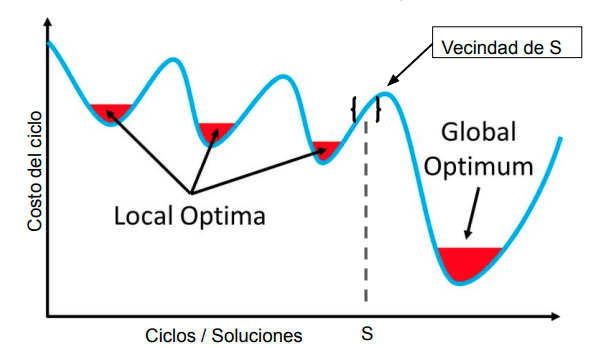
\includegraphics[width=0.5\textwidth]{img/tmp/busqueda-local.png}
    \caption{Esquema representativo del costo de cada ciclo en función de la relación ciclos sobre soluciones. Se puede observar la representación de óptimos locales (local optima), el óptimo global (global optimum) y las soluciones vecinas de $S$.}
    %\label{}
\end{figure}

Para intentar vencer esa limitación se desarrollaron las \textbf{metaheurísticas}, cuyo objetivo es realizar una búsqueda más amplia del espacio de soluciones, para así evitar caer en óptimos locales. Estas no son específicas para un problema dado, sino que son técnicas más generales utilizadas para construir heurísticas de búsqueda particulares para cada uno. La metaheurística implementada en este trabajo es \textbf{Tabú Search}

\subsection{Tabú Search}

La base del método es parecida a búsqueda local, comienza con una solución inicial y se mueve por su vecindad, pero contempla que a veces se necesita pasar por soluciones peores para llegar a soluciones mejores. El problema con esto es que puede llevar a ciclos, entonces para evitarlo hace uso de una \textbf{lista tabú}, que recuerda las soluciones previamente visitadas donde fue y no las exploras nuevamente. El esquema general del método es el descrito en el algoritmo \ref{alg:tabu-esquema}.

\begin{algorithm}[H]
    \begin{algorithmic}[1]
        \State{\textbf{Entrada:} los grafos $G$ y $H$ en representación de lista de adyacencia.}
        \State{\textbf{Salida:} coloreo y su impacto}
        \State
        \Function{TabuSearch}{$G$, $H$, ...}:
            \State actual $\gets$ \textbf{solucionInicial}(G, H) \Comment{$O(I)$}
            \State mejor $\gets$ actual
            \State T $\gets$ \textbf{inicializarMemoria(...)} \Comment{$O(T)$}
            
            \While{No se cumple el \textbf{criterio de parada}} \Comment{$O(\#it)$}
                \State actual $\gets$ $max$\{ filtrarTabu(\textbf{vecindad}(actual), T) \} \Comment{$O(|V| + N(s))$}
                \State T $\gets T + actual$ \Comment{$O(1)$}
                \If{impacto(actual) $>$ impacto(mejor)}
                    \State mejor $\gets$ actual
                \EndIf
            \EndWhile
            \State{\textbf{return} mejor, impacto(mejor)}
        \EndFunction
    \end{algorithmic}
    \caption{Esquema general de tabú search, en \textbf{negrita} cosas a definir. Las complejidades suponen accesos en tiempo constante a memoria}
    \label{alg:tabu-esquema}
\end{algorithm}

La complejidad entonces será $O(I + T + \#it \times (|V| + N(s))$, donde

\begin{itemize}
    \item \textbf{I} es el costo de obtener la solución inicial,
    \item \textbf{T} es el costo de inicializar la memoria,
    \item \textbf{$|V|$} es el tamaño de la vecindad, $max$ y $filtrarTabu$ son lineales en cuanto a ella,
    \item \textbf{N(s)} es el costo de encontrar la vecindad.
\end{itemize}

\subsubsection{Parámetros}

Como se puede ver en esquema general presentado en el Algoritmo \ref{alg:tabu-esquema}, el método varía según la elección de \textbf{solución inicial}, \textbf{memoria}, \textbf{criterio de parada} y \textbf{vecindad}. Se describen las versiones que se contemplan de cada uno.

\begin{itemize}
    \item \textbf{Solución inicial}: Se consideran como procedimientos para generar la solución inicial todas heurísticas constructivas golosas presentadas previamente: W, WP y S-LF.
    \item \textbf{Criterio de parada}: Se toma una cantidad máxima de iteraciones para el algoritmo.
    \item \textbf{Memoria}: Existen dos tipos. Por \textbf{solución} (i.e un coloreo) y \textbf{estructura}, en lugar de recordar las soluciones, se recuerdan los \textit{cambios estructurales} que llevaron de una a otra. En el segundo caso, podría causar que más de una solución que se obtenga con el mismo cambio se marque como tabú y no se visite. Incluso las no exploradas que podrían llegar a ser mejores, dado que el coloreo resultante de aplicar un cambio estructural depende del \textit{contexto} en el cuál se aplicó. El mismo cambio engloba a más de un coloreo. Para evitar perder buenas solucionas, se introduce la \textbf{función de aspiración}. Si una solución es tabú pero es mejor que lo visto hasta el momento, \textit{se aspira} y se la considera como solución factible. Esto es contemplado en \textit{filtrarTabu} del Algoritmo \ref{alg:tabu-esquema}.
    
    Es importante notar que la función de aspiración no tiene sentido junto con la memoria por soluciones, ya que si el algoritmo ya pasó por esa solución, fue contemplada ella y su vecindad en su totalidad, y no tendría sentido volver a verla.
    
    Además, la memoria tiene un tamaño fijo, ya que guardar el espacio entero de soluciones sería demasiado costoso.

    \item \textbf{Vecindad}: Se definen dos movimientos o cambios estructurales para pasar de una solución a otra: \textbf{change} (cambiar un color de un vértice por uno ya usado en el coloreo) y \textbf{swap} (intercambiar los colores de dos vértices). Finalmente, la vecindad de una solución será el conjunto de variaciones que presenten un coloreo válido luego de realizar un solo cambio. Opcionalmente, se puede tomar una parte de la vecindad para restringir la búsqueda e influenciar la toma de decisiones subóptimas. La representación de la estructura utilizada para almacenar en la memoria es en tuplas $(v, c) \mid v \in V, c$ color para $change$ y $(v, w) \mid v, w \in V$ para $swap$.
\end{itemize}

\subsection{Vecindades}

Los procedimientos para las vecindades a ser usados en las implementaciones concretas de Tabú Search son los siguientes:

\begin{algorithm}[H]
    \begin{algorithmic}[1]
        \Function{VecinosChange}{$G = (V, X_G)$, $H$, coloreo, ...} \Comment{$O(n^2 + n \times (m_G + m_H))$}
            \State vecinos $\gets \{\}$
            \For{v $\in$ V} \Comment{$O(n^2 + n \times (m_G + m_H))$}
                \State coloresAdy $\gets \{ coloreo[w] \mid (w, v) \in X_G\} \cup \{ coloreo[v] \}$ \Comment{$O(m_G)$}
                \State coloresFactibles $\gets coloreo \setminus coloresAdy$ \Comment{$O(n)$}
                \For{c $\in$ coloresFactibles}
                \State vecinos $\gets$ vecinos $\cup\ \{(coloreo[v] \twoheadleftarrow c, impacto(coloreo) + \Delta_I\}$ \Comment{$O(m_H)$} \label{alg-line:vecinos-twohead}
                \EndFor 
            \EndFor
            \State \textbf{return} vecinos
            \EndFor
        \EndFunction
        \Function{VecinosSwap}{$G = (V, X_G)$, $H$, coloreo, ...} \Comment{$O(n^2 + n \times (m_G + m_H))$}
            \State vecinos $\gets \{\}$
            \For{v $\in$ V} \Comment{$O(n^2 + n \times (m_G + m_H))$}
                \For{w $\in$ V}
                    \State $swapValido \gets \begin{aligned}[t]
                        &\nexists\ u \in N(v), coloreo[u] = coloreo[w]\ \wedge \\
                        &\nexists\ u \in N(w), coloreo[u] = coloreo[v]
                    \end{aligned}$  \Comment{$O(m_G)$}
                    \If{swapValido}
                        \State vecinos $\gets$ vecinos $\cup\ \{(swap(coloreo, v, w), impacto(coloreo) + \Delta_I\}$ \Comment{$O(m_H)$}
                    \EndIf
                \EndFor
            \EndFor
                
            \State \textbf{return} vecinos
            \EndFor
        \EndFunction
    \end{algorithmic}
    \caption{Procedimientos para distintas vecindades}
    \label{alg:tabu-proc-vecindad}
\end{algorithm}

Donde $\twoheadleftarrow$ en la línea \ref{alg-line:vecinos-twohead} de Change asigna el color al coloreo y devuelve el coloreo resultante. $\Delta_I$ es la diferencia de impacto resultante del cambio estructural. Para ambos casos, se calcula en $O(m_H)$ y está definido de la siguiente manera

$$\Delta_I = \#\{w \in N_H(v) \wedge c_w = c\} - \#\{w \in N_H(v) \wedge c_w = c_v\},$$

donde $c_v$ es el color del vértice $v$, $N_H(v)$ son los vértices adyacentes a él en $H$ y $c$ el nuevo color del vértice $v$.

El tamaño de ambas vecindades $|V|$ es $O(n^2)$, ya que para cada vértice se puede cambiar el color por todos los usados hasta el momento (a lo sumo $n$) o intercambiar con el resto (también $n$).

Para ambas, opcionalmente se puede especificar un \textbf{porcentaje} a tomar de la vecindad, para lo cual se mezcla la vecindad de forma aleatoria y se toma la primera fracción cuyo tamaño alcanza dicho porcentaje. Esto puede ayudar a que tabú explore más y tome soluciones peores que los óptimos locales.

\subsection{Variaciones}\label{ts-variaciones}

Finalmente, se presentan las variaciones de \textit{tabú search} implementadas en este trabajo. Para la complejidad, se deja sin determinar aquello que depende de meta parámetros no definidos, cada uno de los cuales será optimizado durante la experimentación. Por lo tanto, la complejidad es la misma para todos: $O(I + T + \#it \times (|V| + N(s)) = O(I + |T| + \#it \times (n^2 + n \times (m_G + m_H))$

\begin{itemize}
    \item \textbf{TSC-E}: Tabú Search con vecindades de \textit{change} y memoria de tipo estructura.
    \item \textbf{TSC-C}: Tabú Search con vecindades de \textit{change} y memoria de tipo solución (coloreo).
    \item \textbf{TSS-C}: Tabú Search con vecindades de \textit{swap} y memoria de tipo solución (coloreo).
    \item \textbf{TSS-E}: Tabú Search con vecindades de \textit{swap} y memoria de tipo estructura.
\end{itemize}

Cada clase de vecindad tiene una desventaja. Para \textbf{change}, como se cambia el color de un vértice por otro ya utilizado en el coloreo, en cada paso la cantidad de colores pasa a ser menor o igual. Esto hace que el espacio de soluciones al que se puede llegar desde la vecindad de la solución actual se reduzca en cada iteración hasta que no haya más vecinos. Por lo tanto, ciertas soluciones muy cerca del óptimo no se podrían explorar mucho y el algoritmo terminaría cortando luego de pocas iteraciones. En cambio, resulta evidente que algoritmos que den soluciones razonables, pero no con la mínima cantidad de colores, pueden hacer que el algoritmo performe mejor. Por otro lado, en \textbf{swap} pasa lo contrario. Al intercambiar los colores de dos vértices, la cantidad de colores se mantiene luego de cada iteración, por lo que se cree que puede ser más conveniente tener como solución inicial un coloreo de pocos colores. Visto en términos de los algoritmos descritos, probablemente sea conveniente que comience con $S-LF$ o $WP$ en vez de $W$, ya que dan soluciones con menos colores. Estas suposiciones se validarán experimentalmente.